\section{Metodologia}

\subsection{RQs e obiettivi del lavoro}

Le \textbf{RQs} (Research Questions) sono le domande di ricerca che si vogliono risolvere con il lavoro. Queste sono state definite in fase di progettazione del lavoro e sono state utilizzate per guidare lo sviluppo del progetto. Le RQs sono le seguenti:
\begin{itemize}
    \item \textbf{RQ1}: Qual è il trade-off tra emissioni e performance dei modelli di raccomandazione a stato dell'arte?
    \item \textbf{RQ2}: Lavorare con un criterio di early-stopping basato anche sulle emissioni migliora il trade-off tra emissioni e performance rispetto ad un criterio di early-stopping basato sulle sole performance?
    \item \textbf{RQ3}: Quali criteri di early-stopping basati sulle emissioni possono essere utilizzati per migliorare il trade-off tra emissioni e performance dei modelli di raccomandazione a stato dell'arte?
\end{itemize}

\noindent Con la prima RQ si vuole dunque analizzare il trade-off tra emissioni e performance dei modelli di raccomandazione a stato dell'arte. Per rispondere a questa domanda si è deciso di addestrare diversi modelli di raccomandazione a stato dell'arte e di analizzare le emissioni e le performance di ognuno di essi. Con la seconda RQ si vuole invece analizzare se lavorare con un criterio di early-stopping basato anche sulle emissioni migliora il trade-off tra emissioni e performance rispetto ad un criterio di early-stopping basato sulle sole performance. Per rispondere a questa domanda si è prima di tutto studiato il criterio di early-stopping classico e capire come esso funziona, si è studiato il miglioramento delle performance di epoca in epoca e si è analizzato il trade-off tra emissioni e performance. Successivamente si è implementato un criterio di early-stopping basato anche sulle emissioni e si è analizzato il trade-off tra emissioni e performance di questo criterio. Infine con la terza RQ si vuole analizzare quali criteri di early-stopping basati sulle emissioni possono essere utilizzati per migliorare il trade-off tra emissioni e performance dei modelli di raccomandazione a stato dell'arte. Per rispondere a questa domanda si è deciso di implementare diversi criteri di early-stopping basati sulle emissioni e di analizzare il trade-off tra emissioni e performance di ognuno di essi fissando il dataset utilizzato.

\subsection{Addestamento dei modelli}

Per quanto riguarda l'addestamento dei modelli, si è deciso di addestrare i modelli di raccomandazione a stato dell'arte utilizzando diversi dataset. I modelli di raccomandazione a stato dell'arte addestrati sono i seguenti: ItemKNN, BPR, CFKG, CKE, DMF, KGCN, KGNNLS, LINE, MultiDAE, LightGCN, NFCF, DGCF i quali sono tutti presenti in un framework di raccomandazione a stato dell'arte chiamato \textbf{RecBole} \cite{recbole}.\\
Possiamo dividere questi modelli in due gruppi:
\begin{itemize}
    \item \textbf{Modelli di raccomandazione generali CF}: BPR,CFKG, DMF, KGNNLS, LINE, MultiDAE, LightGCN, ItemKNN. Questi modelli sfruttano le sole valutazioni degli utenti per fare raccomandazioni.
    \item \textbf{Modelli di raccomandazione basati su conoscenza}: CKE, KGCN, NFCF, DGCF. Questi modelli sfruttano sia le valutazioni degli utenti che delle conoscenze aggiuntive (knowledge graph) per fare raccomandazioni.
\end{itemize}
\noindent Dunque questi modelli sono stati scelti in quanto rappresentati delle loro categorie (Collaborative Filtering puro, Deep Learning, Graph Neural Network, Knowledge Graph).\\ 
Sono stati usati dei dataset di dimensioni diverse per poter analizzare il comportamento dei modelli in base alla dimensione del dataset. Durante questo lavoro i dataset utilizzati sono i seguenti: \footnote{https://grouplens.org}{\textbf{Movielens-1m}}, \footnote{https://grouplens.org}{\textbf{Movielens-10m}}, \footnote{https://jmcauley.ucsd.edu/data/amazon/}{\textbf{Amazon-Book}}, \footnote{http://www.cp.jku.at/datasets/LFM-1b/}{\textbf{LFM1b}}. I primi due dataset contengono valutazioni di film, il terzo valutazioni di libri e il quarto valutazioni di canzoni. Questi dataset sono compatibili con il framework RecBole.



\subsection{Tracking delle emissioni}
Per il tracking delle emissioni si è deciso di utilizzare una libreria Python chiamata \footnote{https://mlco2.github.io/codecarbon/}{\textbf{CodeCarbon}}, la quale usa il carbon dioxide equivalent (CO$_2$eq) per il tracciamento.\\
\noindent
Tracciare le emissioni degli algoritmi di raccomandazione è molto importante quando si parla di sviluppo sostenibile in campo Recommender Systems. Ancora oggi si tende a trascurare l'impatto ambientale di un'attività e, in questo ambito, si è molto propensi nell'utilizzare dei modelli molti complessi e pesanti
che richiedono molte risorse per essere addestrati ed eseguti per ottenere delle buone performance. Spesso, però, modelli molto più leggeri e semplici riescono a ottenere delle performance molto simili (se non superiori) a modelli più complessi e il tutto con un impatto ambientale decisamente minore.
Ad oggi CO$_2$eq è il principale indicatore utilizzato da governi e enti per misurare l'impatto ambientale di un'attività.
Il CO$_2$eq è un'unità di misura che esprime l'equivalente in CO$_2$ di tutti i gas serra emessi da un'attività, in modo da poter confrontare l'impatto ambientale di attività diverse.
Una strategia comune per calcolare il CO$_2$eq è quella di moltiplicare tra loro il \textbf{carbon intensity(CI)} e l'\textbf{energia consumata(PC)} dall'attività (nel nostro caso l'esecuzione di algoritmi).



\begin{equation}
    \textit{emission} = \textit{CI}  \cdot \textit{PC}
\end{equation}

\noindent In particolare i valori di CI dipendono dalle diverse fonti di energia utilizzate durante la computazione 
(es. energia solare, energia eolica, etc.). Se \textit{s} è la fonte di energia,  \textit{e$_s$} sono le emissioni per KW/h di energia e \textit{p$_s$}  è la percentuale di energia prodotta dalla fonte s, allora il CI è dato da:
\begin{equation}
    \textit{CI} = \sum_{s \in S} \textit{e$_s$} \cdot \textit{p$_s$}
\end{equation}

\begin{figure}[H]
    \centering
    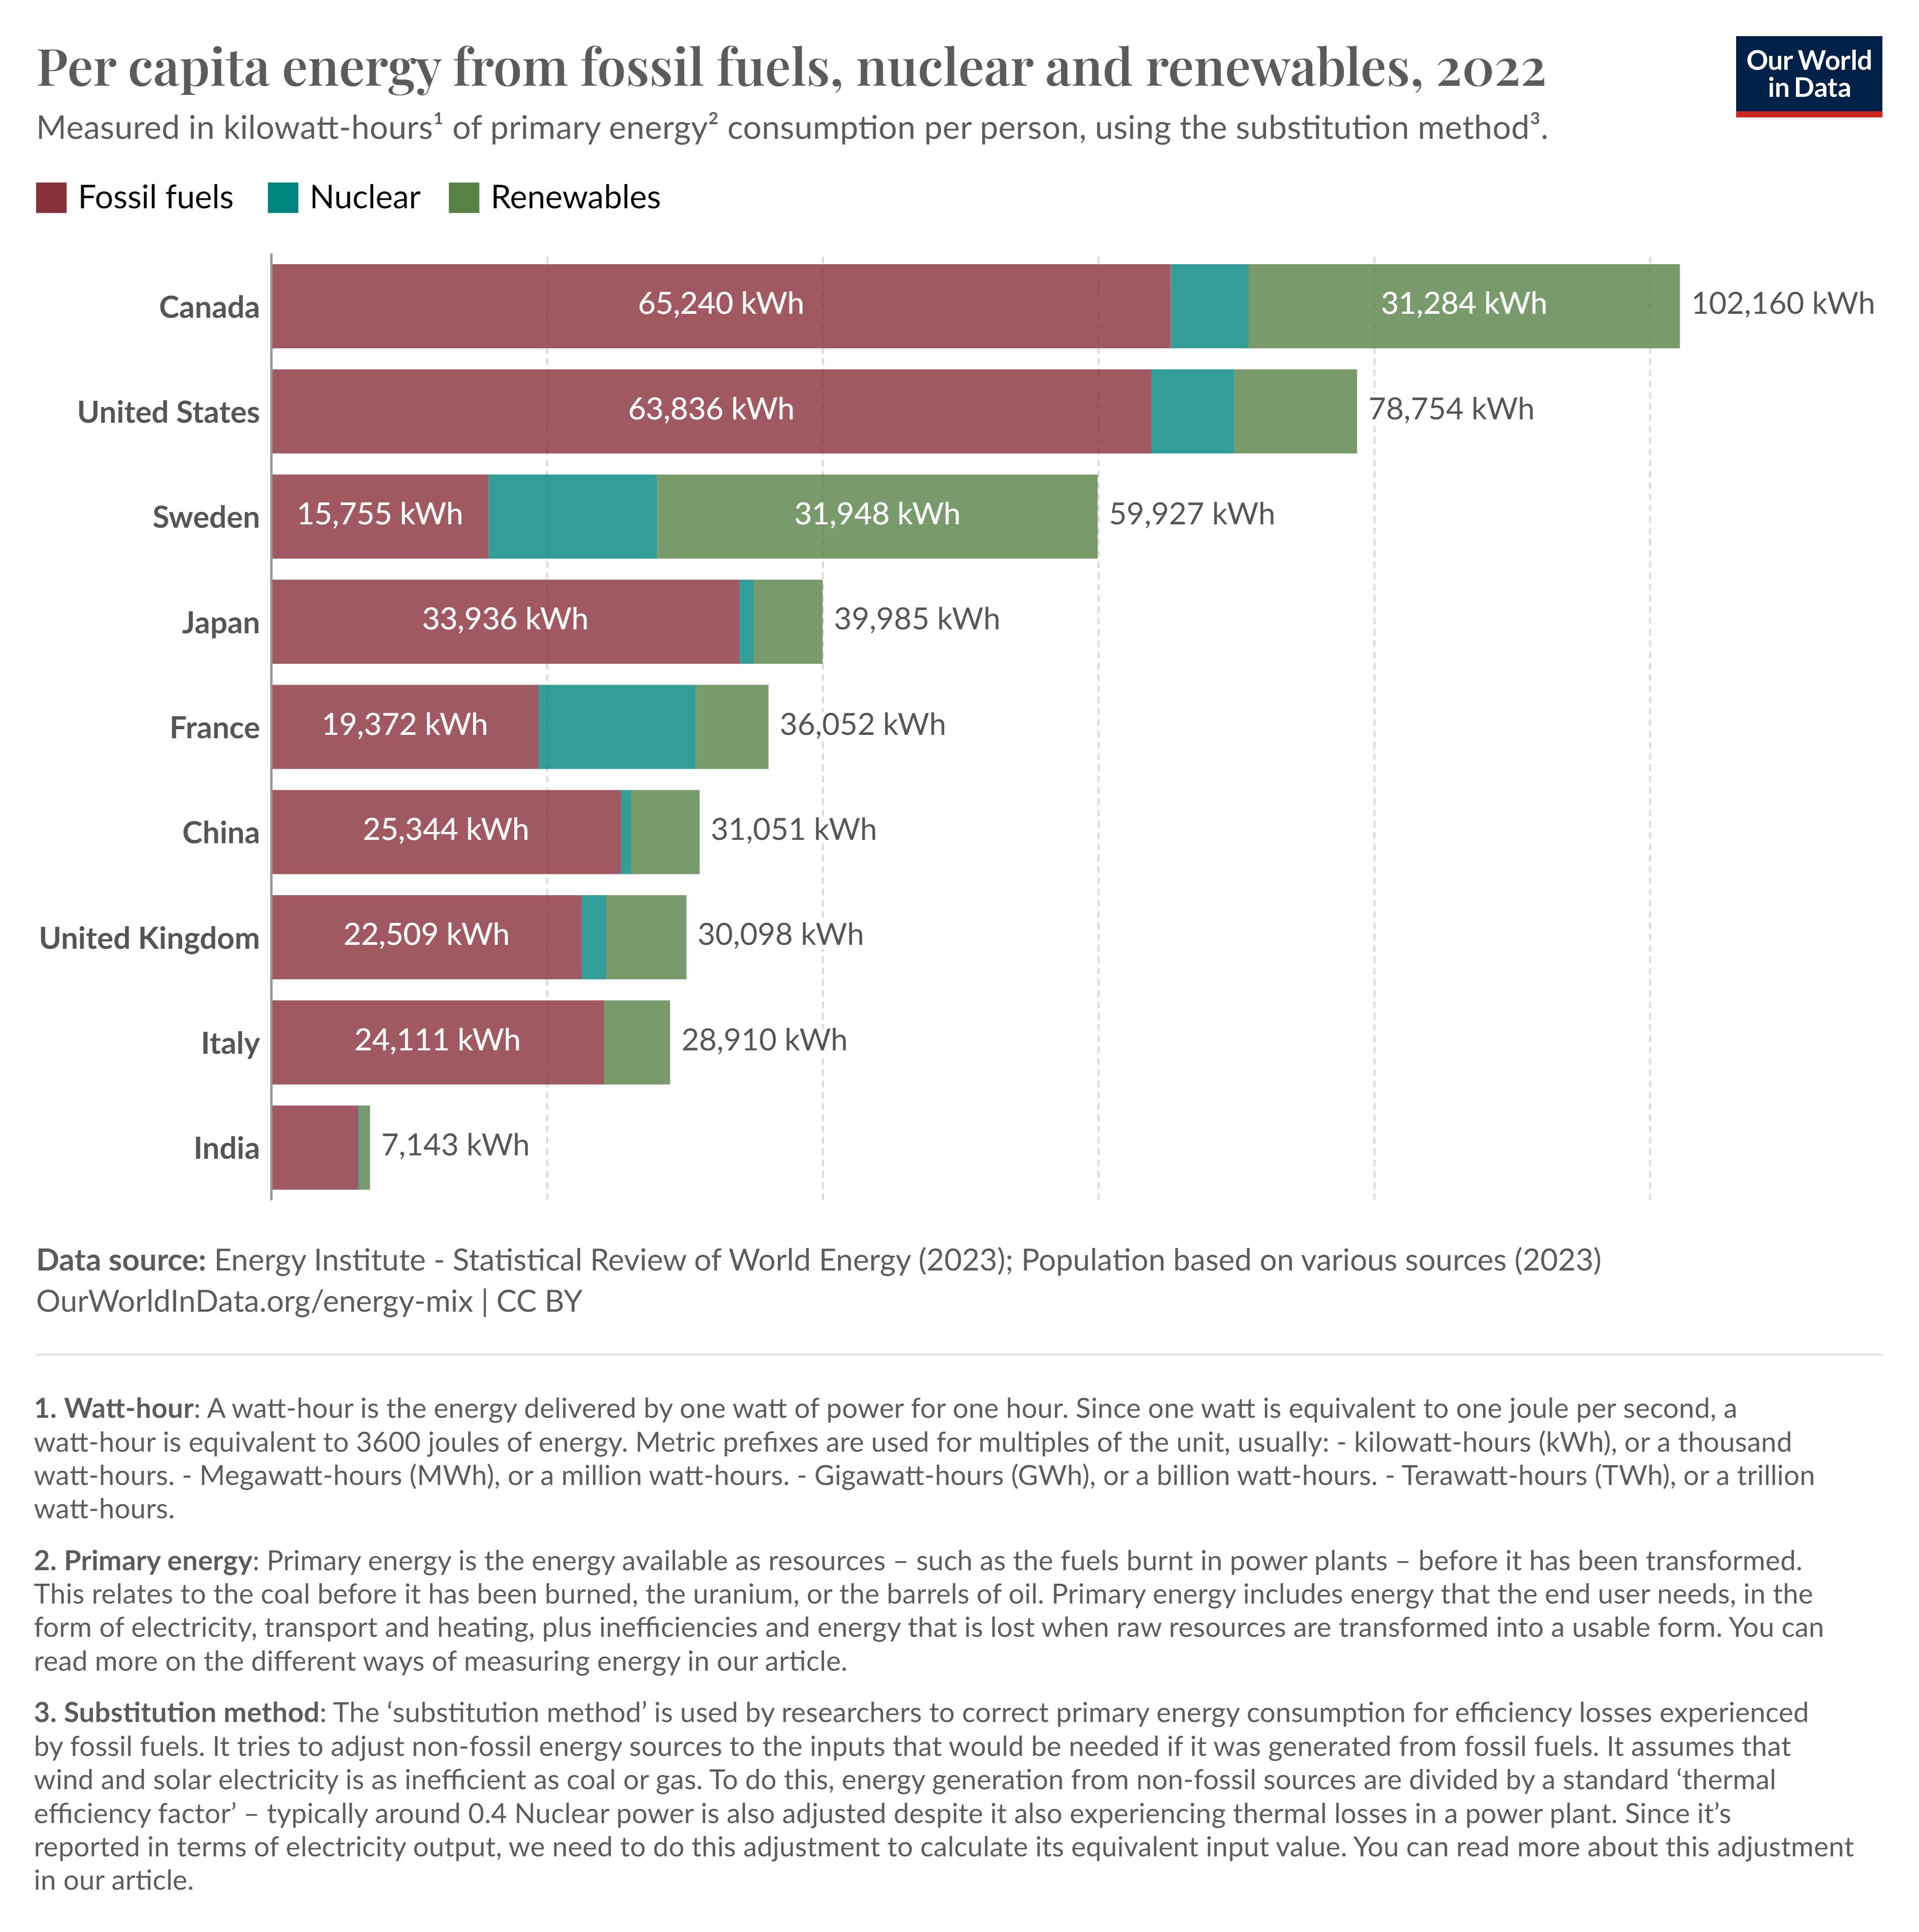
\includegraphics[scale=0.1]{images/per-capita-energy-source-stacked.png}
    \caption{Fonti di energia per paese}
\end{figure}

\noindent Come si può vedere dal grafico \cite{energy-mix} le fonti di energia variano da paese a paese e quindi il CI varia a seconda del paese in cui si esegue l'attività. Questo è un aspetto molto importante nel caso di addestramento sostenibile. A parità di energia consumata un modello addestrato in un paese con una fonte di energia più pulita avrà un impatto ambientale minore rispetto ad un modello addestrato in un paese con una fonte di energia più inquinante.\\
